
% Inledningssektionen

I detta dokument redogörs idéer om hur robotens delsystem kan konstrueras. Det är ej bindande, utan tjänar snarare som en grov kompass inför projektets implementation och planering. Skissen används för att avgöra vilka moduler som ingår och hur arbetet kan delas upp.

\begin{figure}[h!]
    \makebox[\textwidth][c]{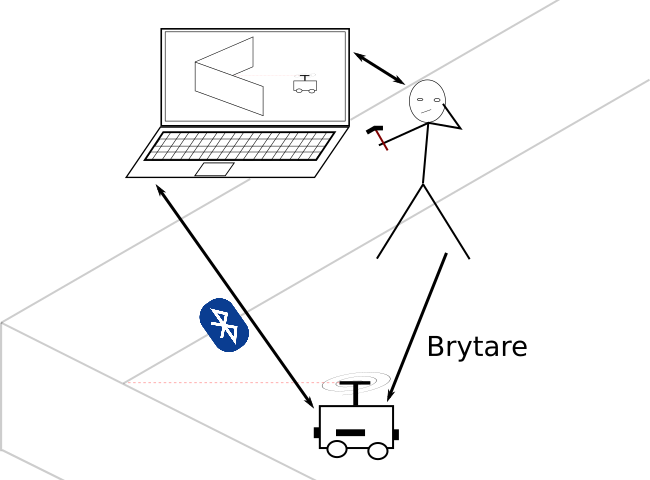
\includegraphics[width=1\textwidth]{overview.png}}
    \caption{Systemet i dess omgivning.}
    \label{fig:overview}
\end{figure}
